\TOWRITE{NT/...}{Finalise}
\TOWRITE{JC}{Proofread concept and approach pass 1
  \begin{compactitem}
  \item Checking whether the overall structure of the narrative
    makes sense
  \item Checking how much this fulfills all the points raised by
    Wolfram
  \end{compactitem}
}
\TOWRITE{ALL}{Proofread concept and approach pass 2 (done by HF)}

\subsection{Concept and Approach}\label{sec:concept}
\eucommentary{5-8 pages}
\eucommentary{
-- Describe and explain the overall concept underpinning the project.
Describe the main ideas, models or assumptions involved. Identify
any trans-disciplinary considerations;
-- Describe and explain the overall approach and methodology, distinguishing, as
appropriate, activities indicated in the relevant section of the work programme, e.g.
Networking Activities, Service Activities and Joint Research Activities, as detailed in
the Part E of the Specific features for Research Infrastructures of the Horizon 2020
European Research Infrastructures (including e-Infrastructures) Work Programme 2014-
2015;\\
-- Describe how the Networking Activities will foster a culture of co-operation between the
participants and other relevant stakeholders.\\
-- Describe how the Service activities will offer access to state-of-the-art infrastructures,
high quality services, and will enable users to conduct excellent research.\\
-- Describe how the Joint Research Activities will contribute to quantitative and qualitative
improvements of the services provided by the infrastructures.\\
-- As per Part E of the Work Programme, where relevant, describe how the project will
share and use existing basic operations services (e.g. authorisation and accounting
systems, service registry, etc.) with other e-infrastructure providers and justify why such
services should be (re)developed if they already exist in other e-infrastructures. Describe
how the developed services will be discoverable on-line.\\
-- Where relevant, describe how sex and/or gender analysis is taken into account in the
project's content.}

%\minitoc

\begin{center}
\begin{boxedminipage}{.95\textwidth}\em
In its briefest form, the concept of this project is to develop,
evaluate and disseminate a
toolkit of compatible, open, modern and powerful software components from
which bespoke VREs can be assembled to meet the needs of research
projects in mathematics and its applications and developed and
maintained by a sustainable free software ecosystem.
\end{boxedminipage}
\end{center}

The next sections explain the history and role of computation in mathematics,
and why our proposed toolkit will meet a wide range of research
needs. We then explore the types of software and software development
model which already exist, in order to explain the remaining tasks
needed to realise our goal, and to maximise impact.

\subsubsection{Background: Mathematics and Innovation in the Digital World}\label{sec:innovation}

\paragraph{Mathematics is at the heart of innovation}\

We live in an innovation-driven society and mathematics is a key enabling tool for
many of those innovations.
%Examples abound.
The global
positioning system (GPS) needs detailed calculations from special and
general relativity.
Computer Assisted Tomography (CAT scanning), a vital medical tool, is based on solving
mathematical inverse problems.
%finite element calculations and
Mobile phone connectivity depends on combinatorial optimization
algorithms and Delaunay triangulations for frequency allocation.
The modern
e-commerce infrastructure relies on cryptographic algorithms
derived from number theory and algebra. At the core of each of these innovations
there is underpinning mathematics developed and implemented as practical
algorithms. These developments have been made possible through investments
into pure and applied research in mathematics over many decades.
Engineering and business innovation then builds on the mathematical
insights to enrich society, though often the
general public remains unaware of their mathematical foundations.


The mathematics research community has always been keen to develop and
adopt new technology, from Newton's innovations in reflecting
telescopes, to Turing and von Neumann's roles as the founding fathers
of Computer Science. The power and adaptability of mathematical ideas
has been applied to generate important technological advances.  In
1945 Alan Turing wrote of his design for the NPL ACE computer, that
``\emph{There will be positively no internal alterations to be made
  even if we wish suddenly to switch from calculating the energy
  levels of the neon atom to the enumeration of groups of order
  720.}''.

This shows both the power of mathematical abstraction, that allowed
two very different problems to be united, and the role of mathematical
research as an ``early adopter'' of computational methods.

Even in more practical areas, such as in web standards, mathematicians
have led the way. MathML was the first XML recommendation, while
\url{planetmath.org} adopted Web 2.0 standards even before
Wikipedia. The theory of high performance computing (HPC) is
underpinned by mathematical models of concurrency. Computer algebra
systems adopted and explored advanced programming concepts like
comprehensions, iterators, or generics long before they became
standard features of modern programming languages (e.g. in the early
seventies for generics in Axiom, versus 2004 for Java).



\paragraph{Digital exploration tools are crucial for research in mathematics}

From their earliest days, electronic computers have been used in pure
mathematics, either to make tables, to prove theorems (famously the
four colour theorem) or, as with the astronomer's telescope, to explore
new theories. Computer aided experiments are now part of the standard
toolbox of the pure mathematician, and certain areas of mathematics
completely depend on it.

Computational experiments have led to new conjectures which have had a
deep impact on the future development of mathematics. An outstanding
example is the Birch and Swinnerton-Dyer conjecture (one of the Clay
Millenium Problems).  Databases relying on computer calculations such
as the Small Groups Library in GAP, the Modular Atlas in group and
representation theory, or the \LMFDB, provide indispensable tools for
researchers. A constructive way of understanding proofs of deep
theorems yields algorithmic tools to deal with highly abstract
concepts. These tools make the concepts available to a broader class
of researchers, with many potential applications. A prominent example
from algebraic geometry is the desingularization theorem of Hironaka,
for which Hironaka won the Fields Medal, and its algorithmization by
Villamayor.

\TOWRITE{SL/JC}{Reinsert language about Serre's conjecture?}
%
% Commented this para out because I don't understand what point it's making
%
%% Spectacular theoretical breakthroughs such as the recent complete
%% resolution of Serre's conjectures, directly inspired by Wiles' proof
%% of Fermat's last theorem, are based on interdisciplinary approaches.
%% % Serre's conjecture was in fact proved completely within the last 10
%% % years, Serre is probably famous enough in Europe (?), and that work
%% % really is a *direct* extension of work of Wiles; at the same time, the
%% % conjecture of Serre and much work on it were directly inspired by big
%% % numerical computations (e.g., by Mestre).
% Current developments on the algorithmic side also allow us to forge
% cross-connections between different areas of mathematics
% computationally, and hence produce cutting-edge applications
% which were previously inconceivable.

\paragraph{Computers as a tool for collaboration not just computation}

Mathematicians have always collaborated openly, and emphasised the
role of the team of authors in a discovery. It is usual to list
authors alphabetically on a paper, rather than the first or last
author getting special credit, and it is normal to write about what
``we'' discovered, rather than assign credit to individuals.
%% An
%% extreme case is the famous footnote ``since completing this work, one of us has died”.
%% \TOWRITE{JC}{can t source this quote -- Sadly neither can I SL}

In the last three decades, however, the mechanisms of collaboration
have changed, and this is enabling a much more widespread and
fine-grained collaboration. Whereas mathematics research on a
day-to-day basis was traditionally a solitary pen-and-paper activity of
talented individuals corresponding via lectures, letters, and journal
articles, it is often now a collaborative, geographically distributed
team activity supported by e-infrastructures.

E-mail was the first step in this direction, allowing correspondence in
seconds instead of days, followed by web based tools such as the
\texttt{arxiv} preprint server, bulletin boards like
\texttt{mathoverflow.net} and collaboration tools such as \SMC\ 
(see Section~\ref{linked-projects},  page~\pageref{sec:SMC-page}), Google
Docs and \texttt{github}.




\paragraph{Collaboration on mathematical software, data,
  knowledge}%\label{}

\TOWRITE{NT}{Why is the next bit in a box? Couldn't it be normal text?}
\begin{center}
\begin{boxedminipage}{.95\textwidth}\em
Today research in many subjects is transformed by the availability of
vast amounts of research data on the Internet. In this area
mathematics has perhaps lagged behind, especially so when it comes to
open exchange of data, not just static publication.  Mathematical data
is very varied and often has a complex structure. It could be divided into
three kinds:
\begin{compactitem}
\item $\mathcal{D}$: tables or lists of numerical or symbolic data
\item $\mathcal{K}$: knowledge about the mathematical objects given as statements
  (definitions, theorems or proofs; either formal or rigorously informal)
\item $\mathcal{S}$ : software that computes (with) the mathematical objects
\end{compactitem}

All three kinds of ``data'' are equally important for mathematics and are tightly
interlinked:
\begin{compactitem}
\item $\mathcal{D}$ serves as examples for $\mathcal{K}$ or as counterexamples for
  conjectures in $\mathcal{K}$;
\item $\mathcal{S}$ computes $\mathcal{D}$ and establishes properties of $\mathcal{D}$
  (given as $\mathcal{K}$);
\item $\mathcal{D}$ tests $\mathcal{S}$, $\mathcal{S}$ is verified with respect to
  $\mathcal{K}$;
\item theorems and proofs in $\mathcal{K}$ induce and justify algorithms for
  $\mathcal{S}$;
\item $\mathcal{D}$ induces conjectures and guides proofs in $\mathcal{K}$.
\end{compactitem}
\end{boxedminipage}
\end{center}
Figure~\ref{fig:thebigpicture} on
page~\pageref{fig:thebigpicture} shows some relationships between
existing mathematical resources of these kinds.

Relevant examples include:
\begin{compactenum}
\item \textbf{Data Repositories/Communities}: Many communities have been collecting and
  sharing data about the objects they study: e.g.
  \begin{compactenum}[a.]
  \item The \emph{Open Encyclopedia of Integer Sequences} [\url{http://oeis.org}] has
    collected sequences of integers for half a century, it now contains publications
    about, relations between, programs for, and data on ca. 250.000 sequences and is
    steadily growing
  \item The \emph{database of L-Functions, Modular Forms, and
    related objects} [\url{http://www.lmfdb.org}] is an extensive
    database of mathematical objects
      arising in Number Theory.  The associated website aims to become
      a modern handbook including tables, formulas, links, and references,
      to these objects, including specific L-functions and their sources.
  \item \FindStat [\url{http://www.findstat.org/}] is an online database for statistics and
  maps on combinatorial objects. Its purpose is to automatically find
  relations between mathematical objects. It was initiated in 2011 and
  contains 228 statistics over 17 classes of objects.
\item The libraries of small groups and semigroups (in \GAP) which
  make accessible complete classifications of key algebraic objects up
  to a certain size.
  \end{compactenum}
\item \textbf{Knowledge Sources and Repositories} There are many ways to represent
  mathematical knowledge and involve computers. Systems and resources range from
  relatively traditional pre-publication systems like
  \begin{compactenum}[a.]
  \item the \emph{Cornell EPrint archive} [\url{http://arxiv.org}] has over 1 million
    {\LaTeX}-based pre-prints of which ca 10-15\% are on mathematics and bordering areas.
  \item via community-driven Q/A sites like [\url{http://mathoverflow.net}] with almost 40
    thousand questions answered
  \item to mathematical encyclopedias like [\url{http//planetmath.org}], which as a Web2.0
    site predates Wikipedia,
  \item the LMFDB website [\url{http://www.lmfdb.org}]  which includes novel ways to present this data, following a principle called \emph{transclusion},
  and in the extreme to
  \item formalizations of mathematical knowledge, e.g., in theorem prover libraries like
    Mizar [\url{http://mizar.org}], which has formalised 50 thousand relatively elementary
    theorems in 40 years or the formalizations of the Feit-Thomson Theorem or the Kepler
    Conjecture.
  \end{compactenum}
\item \textbf{Mathematical Software Development and Systems}
  \begin{compactenum}[a.]
    \item The \GAP library is roughly 400000 lines of code in a
      specially developed high-level language that describes many
      algorithms for diverse computations in algebra and discrete
      mathematics, not all of which are published elsewhere.
  \item A constraint solver such as Minion is by contrast a highly refined
    solution to a single problem (combinatorial search).
  \item The superseeker software provides an enhanced query interface
    to the Encyclopedia of Integer Sequences, detecting when the
    search key is a transformed version of a sequence in the database.
  \end{compactenum}
\end{compactenum}

Many mathematical databases now exist, some very large; however their
internal structure often hides the true richness of the data, limiting
the scope for interaction with it to the specific tasks the designed
had in mind. The past has shown
that a more flexible approach can be  fruitful:
\begin{compactitem}
\item both the Riemann Hypothesis and the Birch and Swinnerton-Dyer conjectures resulted
  from exploratory $L$-function computations, and now stand among the seven Clay Millenium
  Problems;
\item the Monstrous Moonshine conjecture finds its origin in a numerical coincidence
  between dimensions of representations of the Monster group and coefficients of the
  $j$-function, and its conclusion eventually led to Borcherds' Fields medal;
\end{compactitem}


% Comment by William:
% > Regarding "Mathematicians have a strong tradition of sharing knowledge
% > openly", I think one reason for this is that the landscape of math
% > research is arguably *dramatically* larger than the research landscape
% > in any other field.  As a result, mathematicians find themselves in a
% > situation where collaboration is far more rewarding and productive
% > than competition, which results in a basic culture of sharing.  In
% > sharp contrast, in areas like drug discover or physics (or perhaps
% > even more intensely, in business!), being extremely competitive and
% > secretive is frequently the best strategy.  It is thus no surprise to
% > us that mathematicians are leading the way in developing tools for
% > collaboration and sharing.      Of course, many people outside of
% > mathematics simply don't know that there is anything to mathematics
% > "beyond calculus", so they don't realize how broad our research
% > landscape is.
% >
% > I remember a professor in chemistry or physics coming to Sage Days 7
% > at IPAM (UCLA), and remarking that he was very surprised Sage was
% > coming from "number theorists", rather than computer science (say).  I
% > would imagine that computer science is also very competitive, since
% > it's a well-funded area with many people, but compared to mathematics
% > it's basically like one relatively small research area (within
% > combinatorics...).


\paragraph{Computational mathematics is interdisciplinary by nature}


The very name of ``computational mathematics'' suggests that it is
interdisciplinary, drawing on both mathematics and computer
science (and in fact having many applications in physics, chemistry
and engineering as well). Computational techniques also open up
unexpected connections between different areas of mathematics.
For instance fruitful interactions unfold between computer algebra and
algebraic geometry, number theory, combinatorics and group theory. Algebraic algorithms
open up new ways of accessing subareas of these key disciplines of
mathematics, and they are fundamental to practical applications of the
disciplines. Conversely, challenges arising in algebraic geometry, number
theory, combinatorics and group theory quite often lead to algorithmic breakthroughs
which, in turn, open the door for new theoretical and practical applications
of computer algebra.

% +in nature, with links to many areas of mathematics, applications
% +within mathematics and to other branches of science and engineering,
% +and with constantly new and often surprising developments. Many of
% +these developments, and even the creation of whole subareas of the
% +field, have been initiated by European researchers making crucial
% +contributions at all levels. These include the design of fundamental
% +algorithms, the development of major computer algebra systems,
% +applications of the computational methods in various fields, and the
% +creation of widely used databases.



\paragraph{The diversity of needs in the mathematical community}

Certain scientific areas, for example in genomics, have large
communities of researchers whose computational workflows are very
standardised, which justifies the development of specialised Virtual
Research Environments, typically taking the form of clickable web
services. The situation is very different in mathematics.

Indeed mathematical research projects and teams that make use of
computation, databases or collaborative tools are extremely diverse in
size, skills, sophistication, needs, requirements, and available
resources. Here are some typical scenarios to illustrate this:

\begin{compactitem}
\item At one extreme a project might consist of a single researcher, with limited
  general computing expertise, using a computational tool to compute some data
  that confirms or refutes a hypothesis, writing up the results as a paper
  linking to the data and publishing it. Such a user needs a simple system
  that supports the computational tool of their choice, logging and replay of
  the computation, automatic incorporation of key data in a mathematical
  document, data archival and subsequent citation. They will use very little
  computational resource, and probably have no means of paying for what they
  do use, and will have limited ability to install software.

\item A slightly larger research project in, for instance, algebraic
  combinatorics might involve
  two or three researchers of varying computing skills. It will
  require tools from very different areas of mathematics:
  linear algebra, commutative and non-commutative algebra, symbolic
  manipulations, group theory, graph theory, language theory, and
  rewriting techniques, perhaps. The researchers will thus need to use simultaneously many
  computational components, and to implement a specialised library of code
  that combines them in novel ways. They often will have access to
  some local or remote computational resource (cloud or HPC server),
  and parallelization and distribution of the computations is
  essential to cope with combinatorial explosion. Last but not
  least, they will need to visualise the results of their computations,
 typically large graphs
  with complicated information attached to the nodes or edges, and may have
  access to wall-sized screens for this. They will advertise their
  results through lectures involving live demos. Early on, they will
  want to share their code and data with colleagues typically with
  little computing expertise, and eventually contribute it back to the
  community.

\item A larger collaborative project might involve five or six researchers at two
  or three sites, developing a significant extension to a system such as \Sage
  and using it to explore or catalogue examples of the mathematics of
  interest, and publishing multiple versions of their software and data, and a
  number of mathematical papers based upon that data. They need a much more
  sophisticated environment, including communication and collaboration tools,
  software development tools and so on.

\item Yet another type of project would be a very large and open-ended
  collaborative framework such as polymath, but with the capability to attach
  computations, machine-checked proofs and other computational elements to the
  discussion and the collaboratively assembled proof.
\end{compactitem}

These are just a few of the many forms of computational or
collaborative mathematical project that we aim to support.

\subsubsection{Key Concept: a Virtual Research Environment Toolkit}

The diversity of requirements for different projects described above
make it inappropriate to seek to provide  a one-size-fits-all Virtual Research
Environment, not even for substantial subcommunities. Instead we propose:

\begin{framed}
  Toward an Open Digital Research Environments Toolkit for the
  Advancement of Mathematics.

  \TheProject proposes to deliver a flexible \textbf{toolkit} that
  will make it easy for individuals and teams of researchers of any
  size to set up custom collaborative Virtual Research Environments
  tailored to their specific needs, resources and workflows, which
  will provide modern, flexible and reliable support for the entire
  life-cycle of computational and collaborative work in mathematical
  research, from initial exploration to proof, publication, archival,
  teaching and outreach. They will support mathematical computations
  and databases of all scales from tiny to huge.
\end{framed}

The kit will take the form of a collection of compatible components,
ready to be connected using extensible documented interfaces both to
other bespoke components and to standard infrastructural tools and
services. Most of the capabilities of these components will come from
existing software -- computational tools such as \Sage, \GAP,
\Singular and \Pari; databases such as \LMFDB; user interface tools
such as \Jupyter notebooks; existing compute servers, clusters and
clouds; typesetting tools such as \LaTeX\ and so on.

\subsubsection{Benefit of this concept: a Toolkit which can evolve to best support
  real research practices}

The kit will be designed to create VREs that support the ways in which
mathematicians actually work together through the lifecycle of a
project, informed by recent research into the sociology of
mathematical collaboration.

Such engineering of the social aspects of such systems to maximise their
success is an imprecise science. A great deal is learnt from the
deployment of any given system and the reaction of the wider
community. Historically such an experiment has been a massive effort:
\SMC required 70k lines of bespoke code; similarly each of
the databases and collaboration sites is essentially a bespoke
program. Furthermore, much of this effort is necessarily \emph{not} spent on
the innovation in the environment, but on the underlying
infrastructure. Our more flexible and modular system will allow
focus to be placed on the environment
itself. This ability to construct experimental VREs and gain feedback
on them will accelerate the development of  our understanding
of the social dynamics of user and developer communities enormously,
ultimately leading to better VREs.

\subsubsection{Background: the scope of a VRE in mathematics, relevant
  recent developments}

\paragraph{A unifying user interface: executable notebooks and project Jupyter}

\TODO{Maybe some linking text here}

\TOWRITE{Somebody with latex knowledge}{Use wrapfig or so to have text flowing around the figure to savve space.}
\subsubsection{Jupyter}
\label{sec:jupyter}
\TOWRITE{NT}{Where to put this? It contains a description mostly taken  from the WP5 Userinterfaces description that is now moved here and referred to back here. We need to say early on what Jupyter is, and can then refer back to it in the WorkPackages. We just need to put this in the right place in the concept/approach section...}.
\begin{figure}
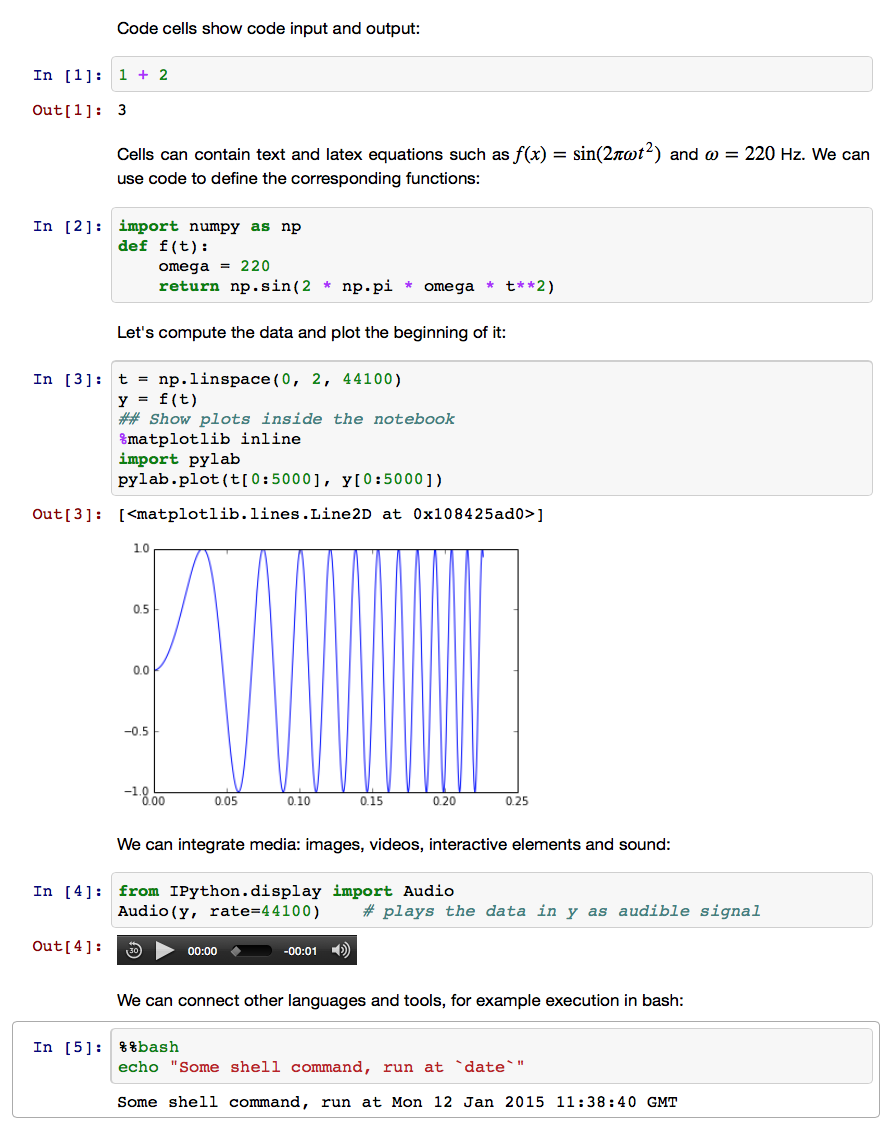
\includegraphics[width=0.6\textwidth]{Pictures/jupyterdemo1.png}
\caption{\label{fig:jupyterdemo} A tiny self-contained Notebook demonstrating the concepts of cells that contain different types of material and can be executed (or updated) in arbitrary or sequential order.}
\end{figure}

Project \Jupyter is a set of open-source software projects for
interactive and exploratory computing. These software projects help
make scientific computing and data science reproducible and
multi-language (Python, Julia, R, Haskell, Bash, R, \ldots). The main
application offered by \Jupyter is the \Jupyter notebook, a unique
web-based interactive computing platform that allows users to create
data- and code-driven narratives that combine live (re-executable)
code, equations, narrative text, interactive dashboards and other rich
media. 

Figure~\ref{fig:jupyterdemo} shows a Python-based sample
session. Within the Python session, all libraries available in Python
can be imported and combined flexibly, a number of interfaces between
different languages exist. Many more examples are available, for
example \cite{IPython-demo-hyperbolic-conservation-laws} and
within \cite{IPython-sload-foundation-report-2013}.

The \Jupyter notebook is being used in all areas of academic
(including for example University of California, Berkeley, Stanford,
MIT, Harvard, Cambridge, Oxford, Imperial College, Southampton,
Hamburg, Paderborn, Vienna, Paris, Katowice, and Oslo) and government
(NASA JPL, LBL, KBase, White House Hackathon) research as well as
industry (Google, IBM, Facebook, Oracle, Otto Group, Microsoft,
Bloomberg, JP Morgan, WhatsApp, O’Reilly, Quantopian, Logilab,
GraphLab, Enthought, Continuum, Authorea, BuzzFeed, etc.)  and
journalism (538, New York Times, etc.). 

Because the architecture and building blocks of \Jupyter are open,
they are being used to build numerous other commercial and non-profit
products and services. The \Jupyter Notebook has between 500,000 and
1.5 million individual users worldwide.

These notebook documents provide a complete and executable record of a
computation that can be shared with others in a way that has not been
possible before. This has led, among other things, to a huge boost in
reproducible, interactive teaching/education documents in recent
years.

We will build on this technology by extending \Jupyter with new
functionality, unifying other computational tools to be usable as
components in this framework, and merging the \Sage and \Jupyter
development.
\TOWRITE{NT}{Is the 'merge' too strong a claim? Please correct / remove.}





\TODO{Here could be a good spot to cite \href{https://www.authorea.com/users/23/articles/8762/_show_article}{The Paper of the Future}}

\paragraph{Virtual Research Environments for Mathematics}\

\begin{figure}
  \centerline{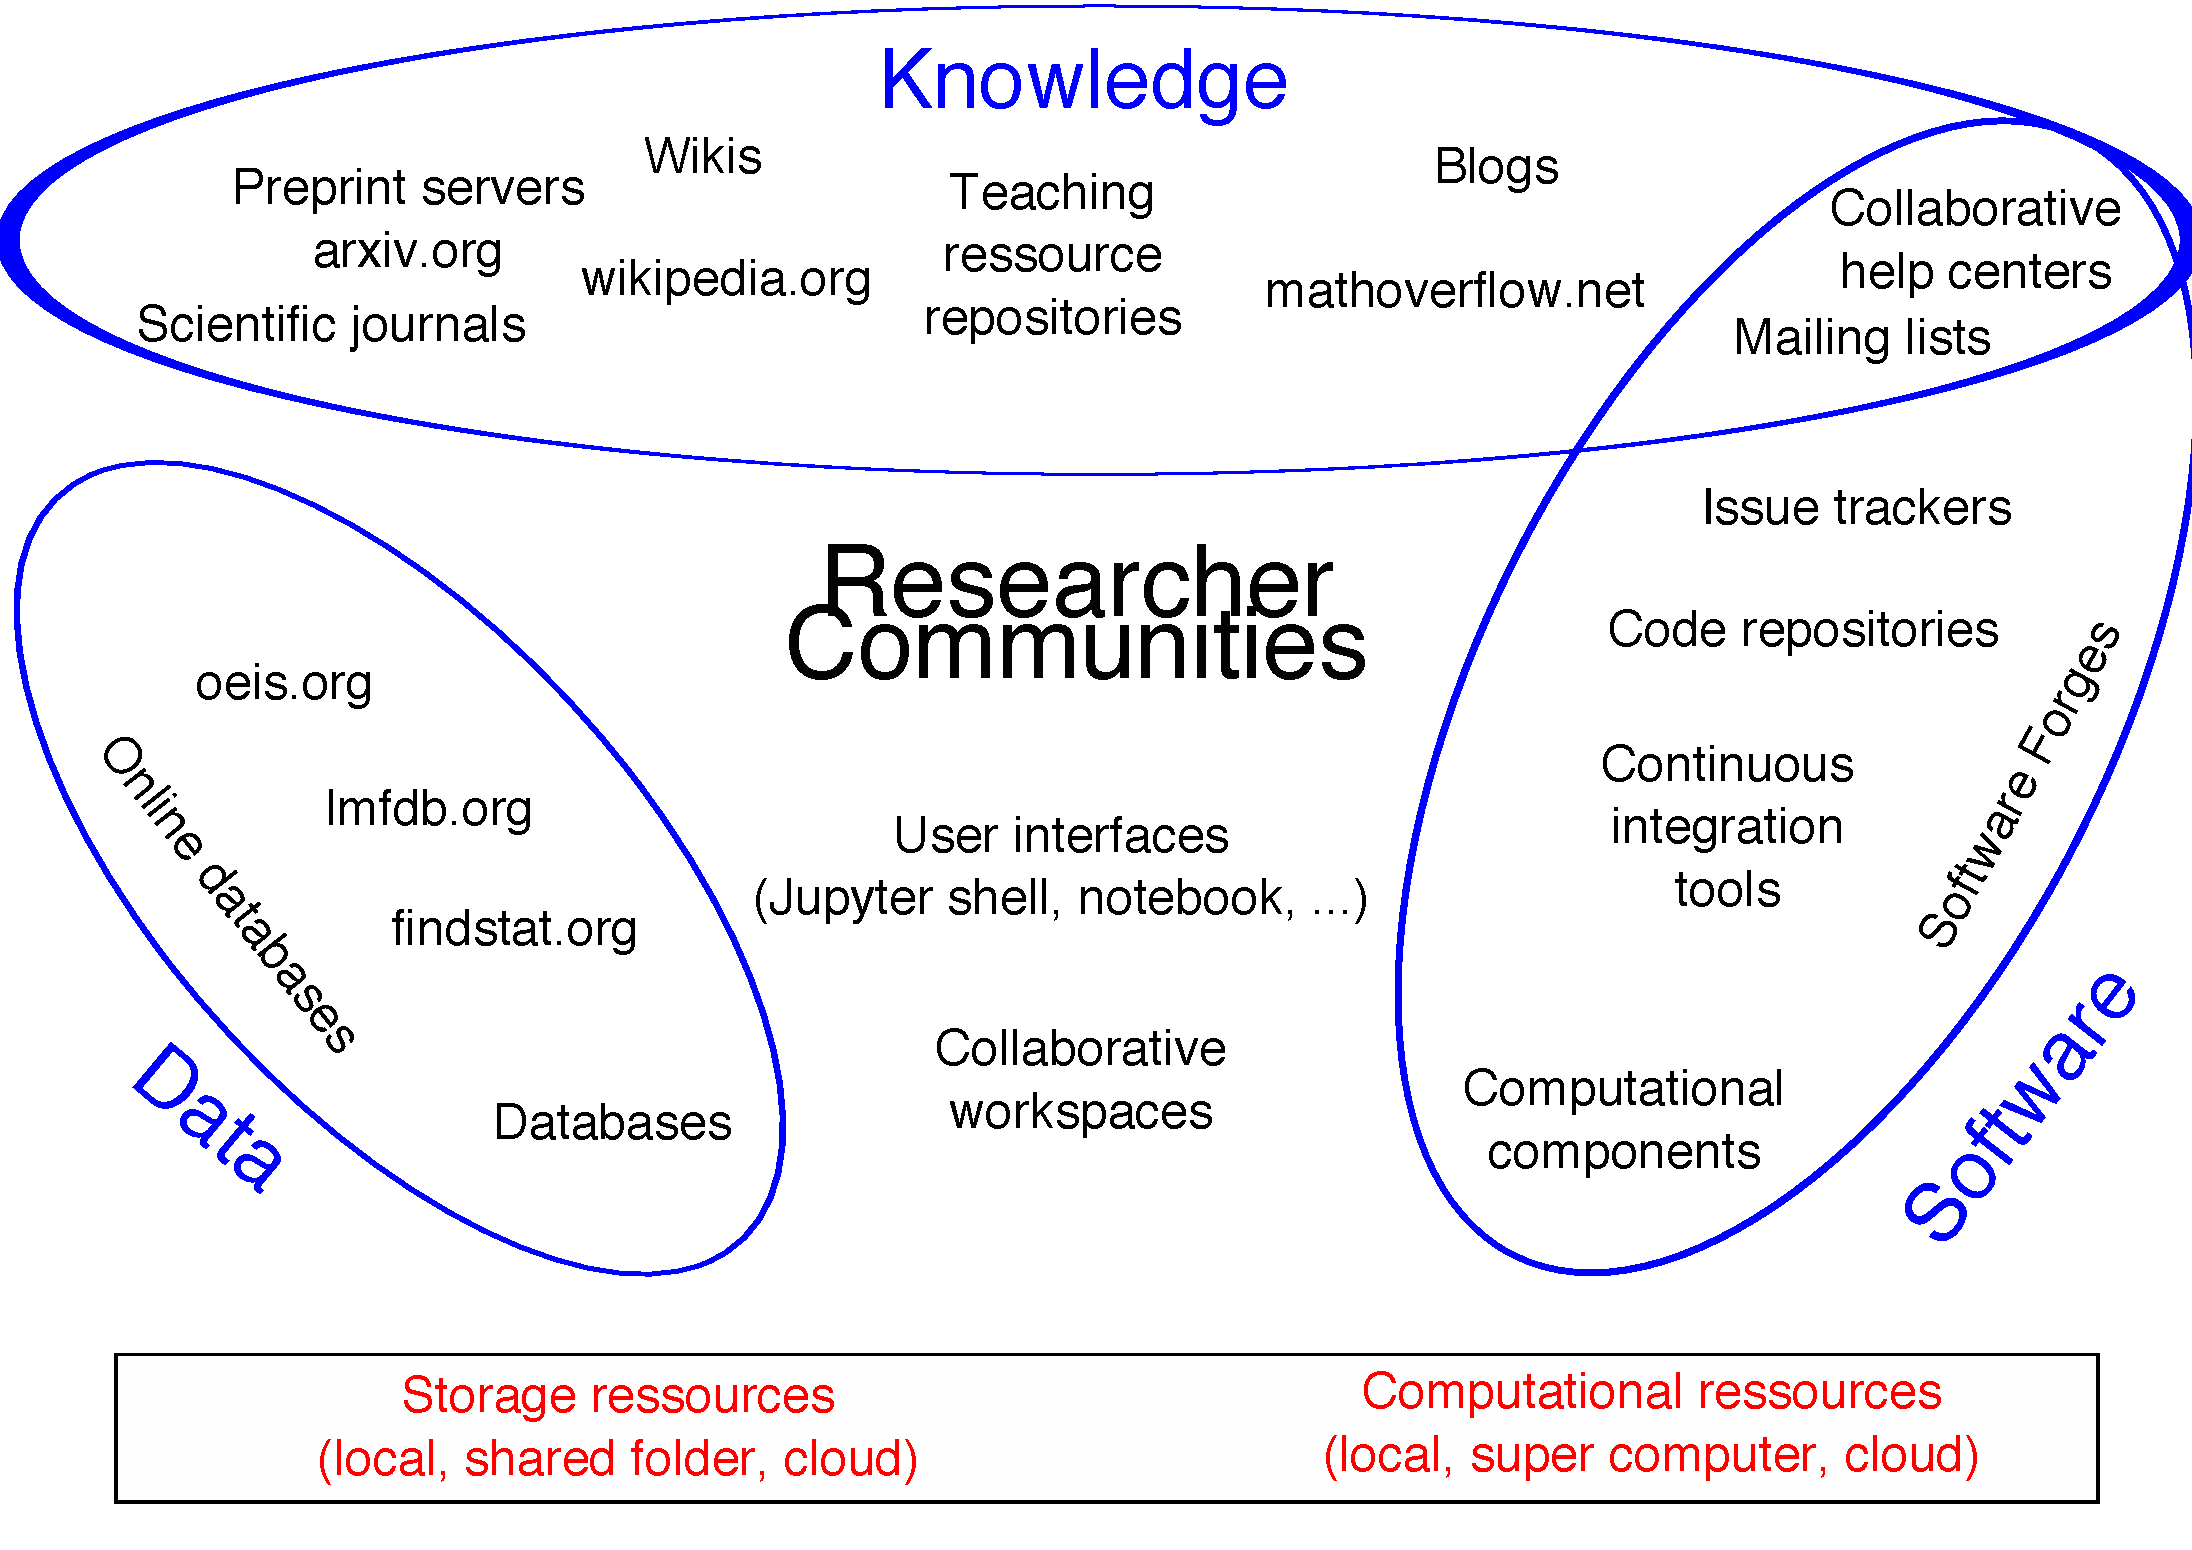
\includegraphics[width=\textwidth]{Pictures/TheBigPicture.pdf}}
  \caption{Virtual Research Environments for research in pure
    mathematics and applications.}
  \label{fig:thebigpicture}
\end{figure}

% \TODO{NT: the purpose of Figure~\ref{fig:thebigpicture} is to give a quick
%   sense of what Virtual Research Environments can be in our context,
%   and a ``big picture'' for the project. A graphic artist friend of
%   mine is going to help me improve it. I have collected here some material for her.\\\\
%   \textbf{\Large What we would like the ``big picture'' in
%     Figure~\ref{fig:thebigpicture} to highlight:}
%   \begin{description}
%   \item[This is a human centered project:] At the core: researchers and communities
%     thereof.
%   \item[The three types of information:]
%     Software, Knowledge, Data (currently in blue)\\
%     How they interact:
%     \begin{compactitem}
%     \item Knowledge help structure data and software (e.g. through ontologies)
%     \item Software produce data
%     \item Data is used by researchers to build knowledge
%     \end{compactitem}
%   \item[Physical resources:]
%     (currently in red)
%   \item[Virtual Research Environments]\ 
%     \begin{compactitem}
%     \item Researchers in Math have a long tradition of collaborating
%       on Software, Knowledge, and, up to some point, Data
%     \item For this they use a variety of collaborative tools which
%       form a loosely knit Virtual Research Environment.
%     \item \textbf{Aim 2}: make it easy for subcommunities of
%       researchers to set up custom collaborative work spaces / Virtual
%       Research Environments tailored to their needs, by combining:
%       \begin{compactitem}
%       \item Computational resources
%       \item Storage resources
%       \item Computational software components
%       \item Databases
%       \item User interfaces
%       \item Wikis-Knowledge bases (true for findstat, LMFDB): quicker
%         cycle for consolidation of information spread over
%         papers/brains
%       \end{compactitem}
%       Such VRE shall help them:
%       \begin{compactitem}
%       \item collaboratively develop software (e.g. specialized
%         libraries), data and knowledge (e.g. articles) for their
%         research projects.
%       \item contribute back this information to the larger community
%         whenever relevant.
%       \end{compactitem}
%     \end{compactitem}
%   \item[Processes:]\ \\
%     It would be interesting to depict the following processes. They
%     are indeed about collaboration and sharing (and quality control),
%     that is what \textbf{Aim 1} is to promote.
%     \begin{description}
%     \item[Software development]\ 
%       \begin{compactitem}
%       \item \emph{bug reports} and \emph{enhancement requests} emerge
%         from the community, typically through collaborative help
%         centers, and are posted on issue trackers.
%       \item \emph{Design discussions} occur on mailing lists and issue
%         trackers.
%       \item Researchers \emph{submit code} to the code repositories.
%       \item \emph{Quality control}: the code is reviewed and
%         tested by continuous integration tools.
%       \item Finally the code \emph{integrated} within computational
%         components, and used by the community.
%       \end{compactitem}
%       Researchers (as well as other users: teachers, engineers, ...)
%       interact at each step of the process.
%     \item[Scientific publication]\ 
%       \begin{compactitem}
%       \item researchers submit articles to journals and post them on
%         preprint servers;
%       \item the articles get reviewed by other researchers;
%       \item finally they are distributed back to the community
%       \end{compactitem}
%     \end{description}
%   \end{description}
%   %
%   Improvements to implement:
%   \begin{compactitem}
%   \item the findstat link does not work for me, kerning looks
%     extremely weird -- POD
%   \item LMFDB, OEIS, and findstat have a strong knowledge component as
%     well, with knowls and wikis, references, ...
%   \item arxiv is not far from a database of knowledge
%   \end{compactitem}
%   %
%   \textbf{\Large A collection of links that might give some idea of
%     the look and feel of our universe:}
%   \begin{description}
%   \item[Examples of (computational) components:]\ 
%     \begin{compactitem}
%     \item IPython: \url{http://ipython.org/}
%     \item GAP: \url{http://www.gap-system.org/}
%     \item Singular: \url{http://www.singular.uni-kl.de/}
%     \item Sage: \url{http://sagemath.org/}
%     \item \PariGP: \url{http://pari.math.u-bordeaux.fr/}
%     \item Linbox: \url{http://www.linalg.org/}
%     \end{compactitem}
%   \item[Examples of online collaborative tools]\ 
%     \begin{compactitem}
%     \item Issue tracker: \url{http://trac.sagemath.org/timeline/}
%     \item Code repository: \url{https://github.com/}
%     \item Collaborative help center: \url{http://ask.sagemath.org/}
%     \item Collaborative math site: \url{http://mathoverflow.net/}
%     \end{compactitem}
%   \item[Examples of online databases]\ 
%     \begin{compactitem}
%     \item Online databases: \url{http://oeis.org/?language=french}
%     \item LMFDB: \url{http://www.lmfdb.org/EllipticCurve/Q/14.a3}
%     \item Findstat: \url{http://www.findstat.org/}
%     \end{compactitem}
%   \item[Example of graphical material]\ 
%     \begin{compactitem}
%     \item \url{http://boxen.math.washington.edu/home/nthiery/main2014.pdf}
%     \end{compactitem}
%   \end{description}
% }


\COMMENT{Role of this section: reflecting our knowledge of the context
  + and explaining that the success of those early VRE’s, even if
  incomplete, showcases their importance and the appetite of the
  community for these kind of tools. It's exciting. We want to
  highlight the appetite rather than the need which is hard to define
  at this point}

%% \begin{center}
%%   \begin{boxedminipage}{.95\textwidth}\em
%%     \COMMENT{In short: maths needs VRE's}

%%     Our priority is the delivery of complete Virtual Research
%%     Environments (VRE). A VRE supports the entire life-cycle of
%%     computational work in mathematical research, from initial
%%     exploration to publication, teaching, and outreach. We envisage
%%     VREs as the main medium for development and deployment of
%%     mathematical research.
%%   \end{boxedminipage}
%% \end{center}

Virtual Research Environments are flexible, powerful, unified
environments for communication, distribution and implementation of
mathematical research.

Initial work shows the potential for this idea, for example, the
Virtual Research and Teaching Environment \SMC\ 
(see Section~\ref{linked-projects},  page~\pageref{sec:SMC-page})
hosting more than 10k users and 100k projects after just one year.  
\SMC is a open-source web-based hosting and web browser-based UI
solution for full access to systems such as \Sage, GAP, Singular, PARI/GP, IPython, and many
more, to the end user, and may be descibed as truly \emph{cloud}-based. 
Figure~\ref{fig:SMC-screenshot} on page~\pageref{fig:SMC-screenshot} shows an example of an SMC session.
\begin{figure}
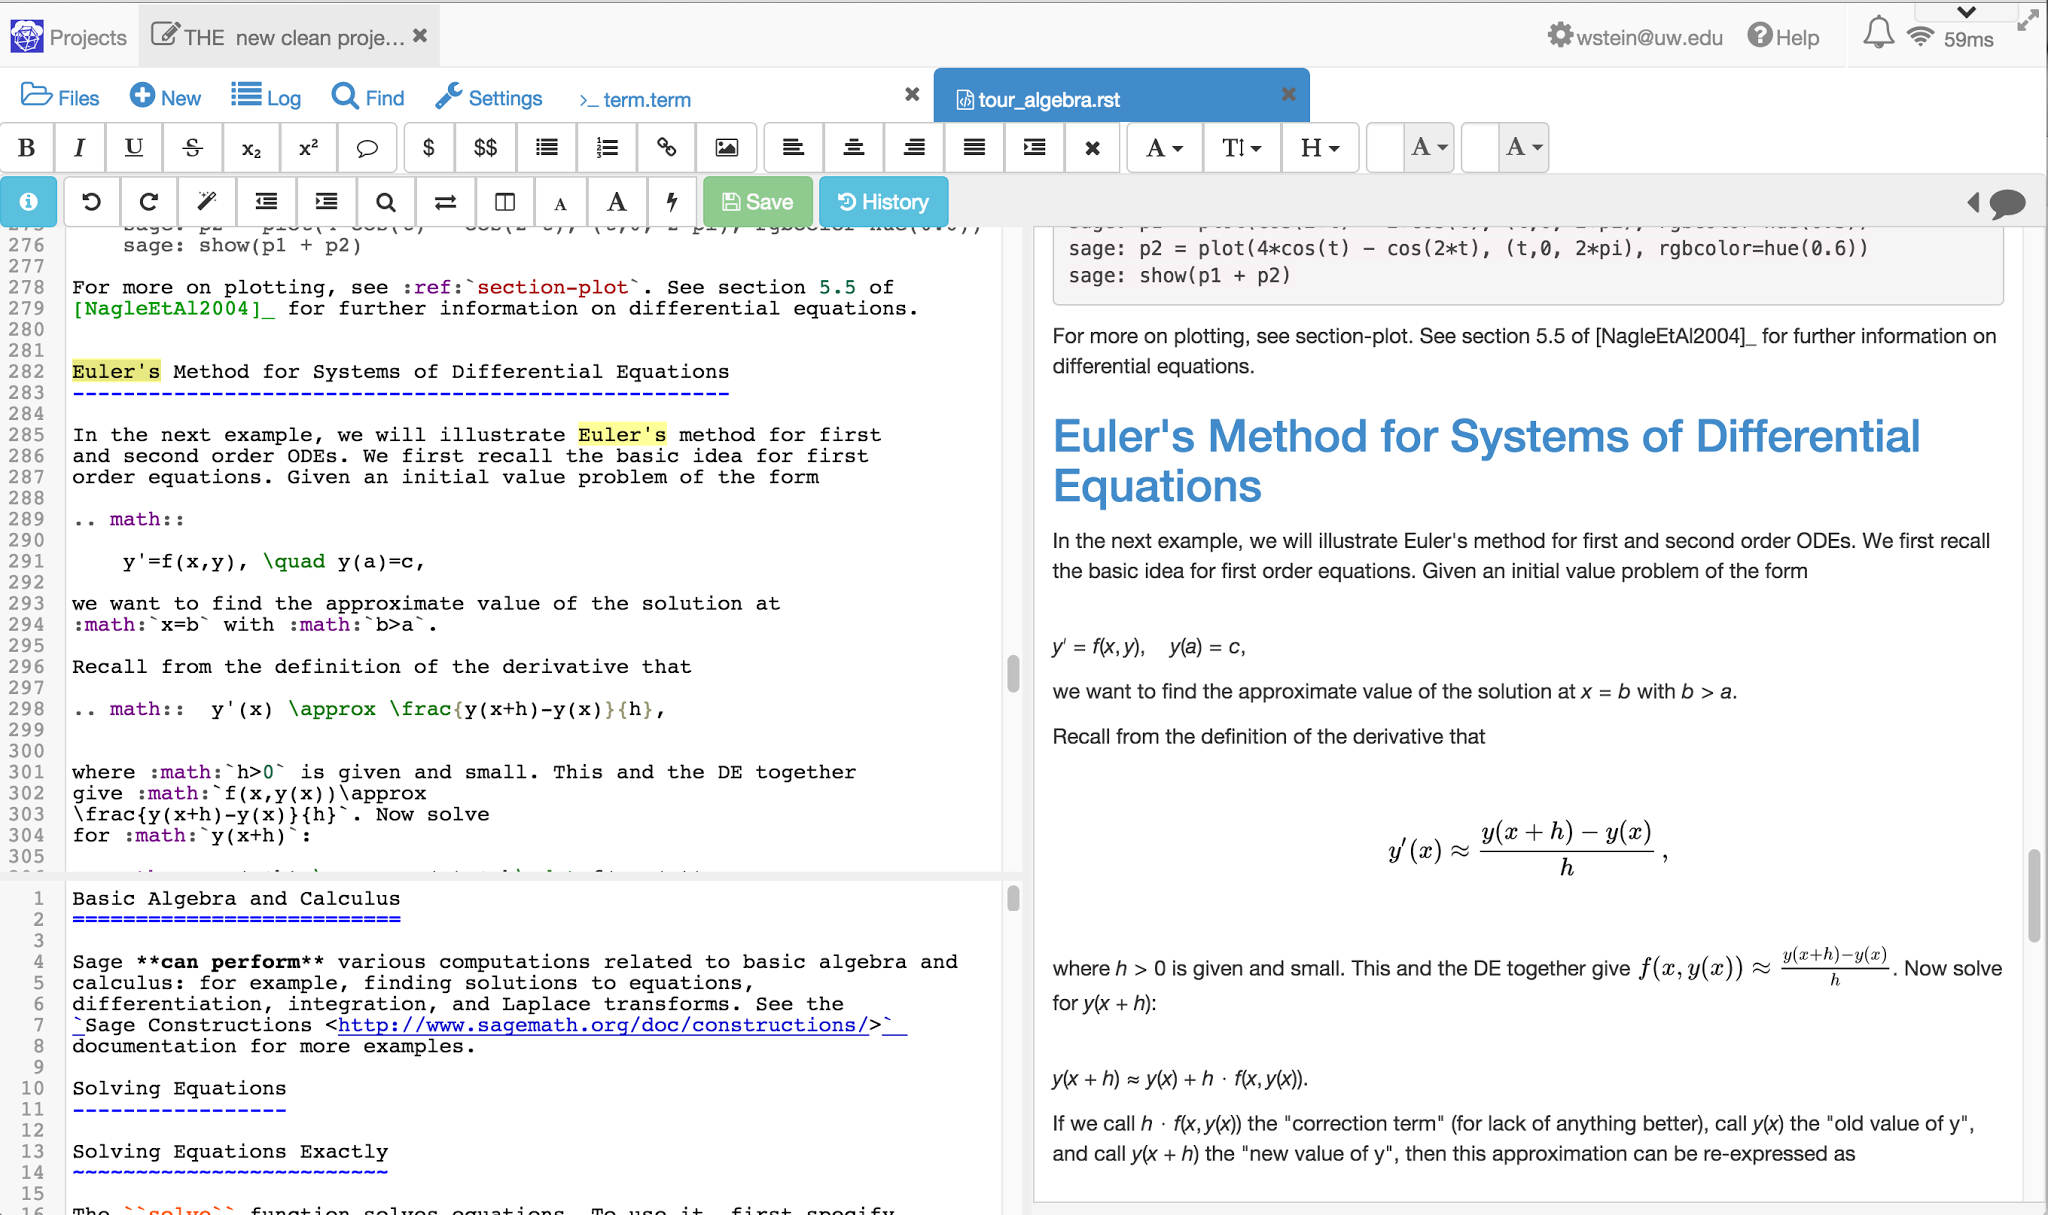
\includegraphics[width=\textwidth]{Pictures/SMC-screenshot.png}
\caption{\label{fig:SMC-screenshot} Typical \SMC\ session in a web browser} 
\end{figure}

There is widespread community interest in well-executed
\emph{integrated solutions} which can enable large-scale collaboration
on Mathematical \emph{software}, \emph{knowledge}, and
\emph{data}. This interest is also evidenced by the considerable
activity (since the inception of the internet) in a range of online
mathematical databases such as the Online Encyclopedia of Integers
Sequences, the Atlas of Finite Group Representations, and \LMFDB.
%
Other systems such as \href{http://polymathprojects.org/}{polymath}
and \href{mathoverflow.net}{MathOverflow} show the interest among
mathematicians in exploring new forms of collaboration, in particular
when the tools are well-designed and the balance of effort and reward
is correct.

Elements of a mathematical VRE can also be seen in ``everyday''
collaboration tools such as \texttt{arxiv} (sharing new mathematical
knowledge with control of provenance) \texttt{Wikipedia} (presenting
established knowledge in a consistent and linked way) and
\texttt{github}, used for collaborative paper writing as
well as software development.

\TODO{Simulagora}


\paragraph{Development models for mathematical software: a historical
  perspective}

Supporting the experimental method in mathematics requires spending
substantial resources
on software development. As the sophistication of the required
computations increased, supported by the growth of available
computational power, it became vital to distribute those efforts across
ever-larger research communities. European mathematicians have been
pioneers in this and have built up a tradition of collaborative open
source software development, that was key
to many highly successful,
open-source, community-developed specialised systems, starting with
\PariGP in Number Theory in 1979, and including \GAP in Group Theory
or \Singular in Algebraic Geometry. This was at a time when much other
scientific computing research relied on bespoke Fortran programs and used
for one calculation and then discarded.
%  \TODO{Is this quite true?
%  \url{http://en.wikipedia.org/wiki/Basic_Linear_Algebra_Subprograms}
%  says BLAS dates back from 1979 as well.}
%
%   Not quite true, but trueish. The NAG library (commercial) is another
%   possible exception

%% \COMMENT{The emergence of massive collaborative development models and
%%   tools is revolutionizing the landscape; innovation is now led by
%%   communities, not corporate software}

%% \TODO{There is redundancy below}

In that period, inter-project communication was limited by the lack of
standardisation of, and interconnection between, computers. Systems
produced remained limited
to specific research topics and often specific computer systems and
were not easily interoperable. It was left to the
corporate world to gather sufficient manpower to develop general
purpose systems that could support a broad range of engineering,
scientific and statistical mathematics, through a coherent user
interface. These companies (e.g., Wolfram, Mathworks, MapleSoft) were
mainly US-based and created a profitable industry.

% The next scale was reached in the last decade with the advent of the
% general purpose mathematical system \Sage which proved the viability
% and sustainability of the ``developed by users for users'' development
% model at the international level.

The modern environment, however, is quite different. A more connected
digital world has led to the emergence of open source software and
open development models (the so-called ``bazaar'' approach). This is
clearly exemplified in the \Sage system. \Sage is a truly
general purpose computational mathematical system. It is committed to,
and draws huge benefits from the power of open source software.
% a virtual software development environment.
It showcases the modern
reality that open source software is not just a viable alternative for
commercially produced alternatives, but it actually allows for more
rapid innovation through providing an open platform through which the
community can deploy and share advances more rapidly. \Sage demonstrates
this modern community approach to development by
delivering high quality software to researchers, teachers, and
practitioners in mathematics. It is founded on a widespread
international community of contributors and developers, and builds
successfully on a large stack of existing open source software,
ranging from the specialised computational systems mentioned above, to
\Python, a general purpose programming language that is used by
millions of programmers worldwide. This flexible, open source
architecture then allows it to rapidly assimilate new components such
as \Jupyter (formerly IPython notebook) as they are developed.

In the 1980s and 1990s the economies of scale favoured the commercial
development model for mathematical software: corporate entities could
co-locate a large body of expertise and orient it towards one
goal. This was difficult for the much larger, but naturally more
dissipated, communities of mathematical researchers. However, modern
interconnection of researchers (through the infrastructure of the
internet and collaborative development environments such as github)
start to reverse the balance of these economies. Commercial packages
can no longer develop fast enough to assimilate the innovation of the
wider mathematical community, where there is greater expertise and
manpower.

%% \TODO{The material here is somewhat redundant with the language in
%%   Objective~\ref{objective:sustainable}; see where this belongs best
%%   to. The previous section being too long, it might be good to move
%%   things here.}



\subsubsection{Approach}

In previous sections, we have analyzed the diverse needs of
researchers in pure mathematics and applications, and argued that the
concept of a VRE toolkit, as proposed by \TheProject, will match those
needs, and have a considerable impact on how mathematical research is
conducted.

In this section we describe how we will realise this concept by
building on existing software components in a new way, and why
this is an ideal time to do so.
\begin{framed}
  The fundamental factor is that the last decade has witnessed the
  emergence of the necessary building blocks, all in open source:
  \begin{compactitem}
  \item Key enabling technologies: virtual machines and containers for easy
    deployment; open cloud infrastructure; web technologies
    such as MathJax or WebGL allowing powerful in-browser clients; scalable
    decentralised database software and more
  \item Computational mathematics components as described elsewhere in
    this proposal
  \item Flexible user interfaces and interactive computing environments
  \end{compactitem}
\end{framed}

The emergence of these components is itself enabled by progress in the
wider technological environment -- cheap powerful computers; fast
reliable networks; stable and advanced platforms such as JavaScript;
and more importantly and uniquely the maturation of open source
development models and collaborative tools (e.g. \texttt{github})
supporting them. This now
makes it possible to  bring together large and diverse communities of
developers, and foster large ecosystems of interoperable
components. We elaborate later in this section how this has
specifically affected the development of mathematical software in the
last decade, showcasing the sustainability of the ``by users for
users`` development models even for general purpose mathematical
computational components. These models are still not perfect on the
largest scales, and we will address this, for our purposes within the project.

\begin{framed}
  Our technical approach is to join forces with the \Jupyter project and focus on developing
  and improving building blocks that can be
  assembled and re-used flexibly to address the varied
  requirements of mathematics and the applications of mathematics in
  science and engineering, rather than creating one particular
  monolithic environment.
\end{framed}
\paragraph{Activities}

The activities of the project are planned and structured to develop
and promote \TheProject, including new research into
architectures, database techniques, parallel algorithms and the
sociology of collaborative free software development, as well as
engineering work on existing software and networking and
community-building activities.

The project inherently spans the disciplines of mathematics and
computer science, as well as bringing in results and techniques from
social sciences. Exemplar applications may also arise from areas to
which symbolic and algebraic computing is applied, such as physics,
chemistry, systems biology and engineering.


The project is divided into seven work packages. Work Package
\WPref{management} covers project management and coordination as
usual. Work Package \WPref{dissem} is our main networking activity
including community-building workshops, demonstrator applications and
direct dissemination of project results.
This covers the following topics from section E of the Work Programme:
\begin{compactitem}
\item dissemination and/or exploitation of project results and
  knowledge, contribution to socioeconomic impacts, promotion of
  innovation (\taskref{dissem}{dissemination-communication},
  \taskref{dissem}{dissemination});
\item reinforcing partnership with industry: outreach and
  dissemination activities, transfer of knowledge, activities to
  foster the use of e-infrastructures by industrial researchers,
  involvement of industrial associations in consortia or in advisory
  bodies (\taskref{dissem}{dissemination-communication},
  \taskref{dissem}{dissemination}, \taskref{dissem}{project-intro});
\item strengthening of virtual research communities
  (\taskref{dissem}{devel-workshops},\taskref{dissem}{dissemination});
\item spreading of good practices, consultancy and training courses to
  new users (\taskref{dissem}{project-intro},
  \taskref{dissem}{dissemination-of-oommf-nb-workshops});
\item exchange of personnel and training of staff
  (\taskref{dissem}{devel-workshops}).
\end{compactitem}


The remaining work packages are Joint Research Activities, dividing up
the research needed to design and implement the \TheProject and
investigate the best models for its future development. \TODO{Explain
  the rationale for the division and how they all come together at the end}

This covers the following topics from section E of the Work Programme:

\begin{compactitem}
\item higher performance methodologies and protocols, higher performance instrumentation,
  including the testing of components, subsystems, materials, techniques and dedicated
  software; (\WPref{UI}, \WPref{hpc})
\item integration of installations and infrastructures into virtual
  facilities (\WPref{component-architecture}, \WPref{social-aspects});
\item innovative solutions for data collection, management, curation
  and annotation (\WPref{dksbases});
\end{compactitem}

\TODO{tasks or WPs}

Additional topics addressed include effective software development and
maintenance methodologies for systems of free software systems and the
design of VREs to best support real mathematical practice.

Since the infrastructure that we are developing is free software,
there is no need for formal Service activities. All partners have
access to all the software anyway, and development and demonstration
can take place on computing resources already available to them.

\subparagraph{Networking activities}
The mathematical software community, and the various overlapping open
source software communities already have an excellent spirit of
collaboration, and excellent cultures promoting open debate, constant
improvement and common purpose. Our networking activities build on
this in essentially two directions: within the project we aim to
provide more opportunities for close collaboration and learning
from one another, in visits, code sprints, and cross-community days;
outside the project we aim to encourage more users of mathematical
computation to join this ``community-of-communities'' through our open
workshops, training events and demonstrator applications.



\subparagraph{Joint Research Activities} The joint research activities are defined by our
vision for \TheProject. \WPref{component-architecture} defines the
requirements for a component to be part of the kit, \WPref{UI}, \WPref{hpc} and
\WPref{dksbases} address limitations of current components, or areas where they have
become out of date and \WPref{social-aspects} is key to our goal to produce systems that
are both effective and sustainable.


By focusing on a toolkit rather than a monolithic VRE, and by
concentrating the efforts on improving and unifying existing general
purpose building blocks, \TheProject
will simultaneously maximise sustainability and broad impact. Although
the primary target users are \emph{researchers in
  mathematics}, the beneficiaries include users of components such as
\Jupyter in  scientific
computing, physics, chemistry, biology, engineering, medicine, earth
sciences and geography, and  teachers
and practitioners in industry as well as researchers.
Users of many of the component systems will also benefit from our
improvements even if they do not choose to use \TheProject VRE, since
those components will be updated and improved. We will also perform
important research into open
development models that will benefit academia and many highly
innovative SME's.


\subsubsection{Benefits of this approach}

Throughout this project we will reuse and extend existing open source
systems. By doing this, we ensure that \TheProject will benefit from future open
source contributions during and beyond the lifetime of the project. By
unifying tools with overlapping functionality, such as \Jupyter and
\Sage, we focus the effort of the computational community onto
\TheProject, producing additional economies of scale. Finally, thanks
to the ``by users for users`` model, the development will be steered
by the actual needs of the community.

The net effect of this is that \TheProject will include far more
capabilities and code than could possibly be developed within a single
research project, and will continue to accrue additional capabilities
from its users as it is used. The investment in this project will be
greatly amplified by these factors and the impact and sustainability
greatly increased.


\subsubsection{Demonstrators}

\TOWRITE{SL}{include the other demonstrators and emphasise links to rest of the project}




\paragraph{Demonstrator: Training and education of the next generation
  computationalists} --- We will produce a series of interactive books
that can be read, executed, modified and explored within the
\TheProject VREs, targetting Biology, Physics, Maths and Engineering
students to demonstate the power of the approach and to train future
scientists and engineers to embrace and exploit these advances in
computational methodology (\taskref{dissem}{ibook}). We will also
create additional materials for teachers at all levels to help them
act as multipliers and disseminate the advances developed here widely~(\taskref{dissem}{project-intro}).
\TOWRITE{SL}{Stephen (?) I have added a first draft for other
  demonstrators (above) - have we got more?, Hans}

\begin{figure}
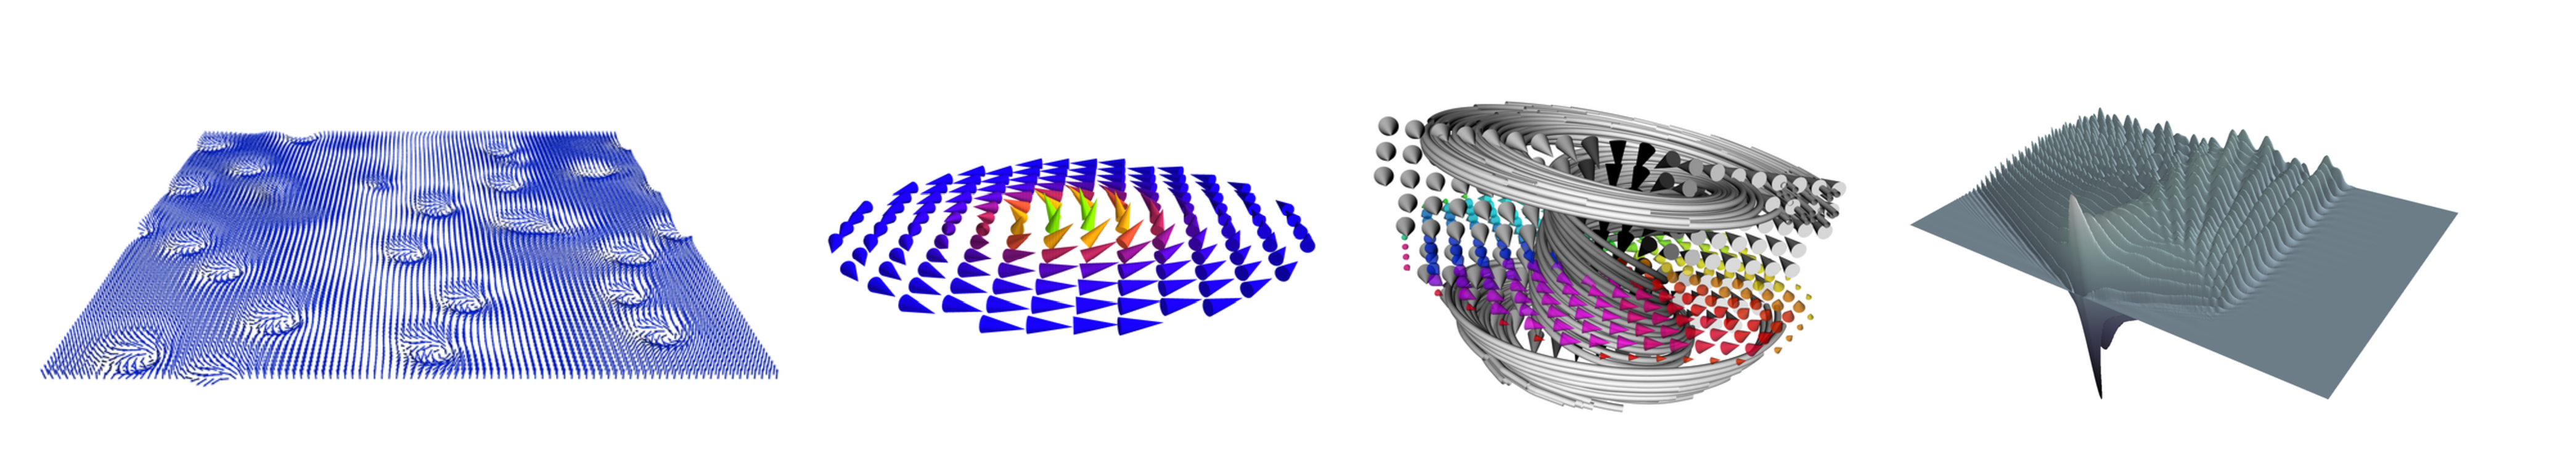
\includegraphics[width=1.0\textwidth]{Pictures/micromagnetic-and-3d-vis-4x1.pdf}
\caption{\label{fig:3d-plots} A selection of typical visualisation patterns often required in science and engineering. From left to right: a 3d vector field on a 2d domain, a 3d vector field coloured with another scalar field on a 2d domain, a 3d vectorfield on a 3d domain with streamlines, and scalar field plotted on a 2d domain.}
\end{figure}

\paragraph{Demonstrator: Micromagnetic VRE}
\label{sec:introduction-micromagnetic-vre-demonstrator}
--- Micromagnetics is a continuum theory description of the behaviour of
the magnetisation vector field at length scales of the order of
micrometers and below. It is widely used in the research and
development of magnetic data storage media and devices, for magnetic
sensing, permanent magnets and healthcare applications such as cancer
treatment and diagnostics. The mathematical model is a time dependent
nonlinear partial differential equation with multiple length and time
scales in the problem, and solution strategies are based on finite
difference and finite element space discretisations and sophisticated
numerical solution of the equations. As in many other research fields,
the groups carrying out the simulations are often not the code
developers, nor have they extensive computational background. More
commonly, these are material scientists, engineers and physicists that
use the simulation to interpret their experiments and support their
device design planning. Industrial users include Seagate, Hitachi,
TDK, Samsung, Bosch and Toyota.

Figure~\ref{fig:3d-plots} shows magnetisation vector fields obtained
in typical micromagnetic studies. They relate, from left to
right, to a set of interacting magnetic skyrmions in a thin flim, a
vortex in a thin Nickel film, a vortex in a half-sphere geometry, and
the propagation of magnetic excitations (only one component plotted)
in a 1d-system.

In this project, we will use the \TheProject components to put
together a in micromagnetic VRE to (i) demonstrate the power of the
approach in a concrete applied research setting, (ii) exploit that
experience to evaluate the real value of the structure of this VRE and
\TheProject to a large and diverse set of end-users.

In more detail, we will embed the most popular micromagnetic
simulation software: the Object Oriented MicroMagnetic Framework
\cite{OOMMF-url} within a micromagnetic VRE, complement this with
value-adding features, develop a substantial number of executable
documents inside this VRE that act as tutorials and documentation,
disseminate the software and documents as open source and through
workshops for the micromagnetic community.  

We have chosen the OOMMF simulation package as the target tool because
it is a somewhat typical representative of computational software:
computation is driven through a text-based configuration file, data
files are produced, and later processed, then figures are created from
the processed data; leaving the scientist with the burden to link all
these elements together. The benefits of moving to the integrated
notebook workflow (see Section~\ref{sec:jupyter}) are
substantial. Furthermore, OOMMF is widely used (over 1800 recorded
publications \cite{OOMMF-citations-url}) and thus provides benefit to
an active and substantial community, who in return will provide plenty
of feedback.

We evaluate the value of this demonstrator
(\taskref{social-aspects}{oommf-nb-evaluation}), immediately feeding
results back into the \TheProject work. This will also
be a case study for the sustainability of the approach and tool beyond
the life time of this H2020 project.




\subsubsection{Specific requests of the call}

\paragraph{Use of Existing Basic Services}
This will be addressed primarily in work packages \WPref{component-architecture},
\WPref{dksbases} and \WPref{hpc}. Our architecture will include interfaces to standard
APIs for cloud provisioning, authentication, cloud storage, HPC scheduling and so
forth. Actual VREs will be deployed by users integrating those with specialist tools
according to the needs of their projects. \COMMENT{weak}

\paragraph{Gender analysis}

All partners will follow inclusive practices in recruiting staff for this project, in
inviting the community to our workshops and outreach events and in choosing users to
evaluate our demonstrator applications. We will consult with the Head of Equality and
Diversity at St Andrews, about any known gender differences in collaborative working and
ensure that our collaborative tools properly support open, equitable and inclusive
patterns of cooperation. This will be reported in deliverable \delivref{management}{ipr}.

\paragraph{Service discovery}

The \TheProject web pages (\taskref{dissem}{dissemination-communication}) and the
dedicated training portal (\taskref{dissem}{training-portal}) will
provide a central point of service discovery, providing a directory to
all components, demonstrators, online services, protocol and interface
specifications, software and other project activities and outputs.

\TOWRITE{NT}{Happy with the above Service discovery snippet?}

%%  \TheProject aims to create a framework to make the
%% systems interoperable and synergistic and to give working mathematicians full access to
%% the potential spanned by already-existing systems. Essentially every node in
%% Figure~\ref{fig:thebigpicture} represents a user community, so \TheProject is at its heart
%% a project that also combines researchers and communities.


%% \subsubsection{Old material}

%% \TODO{What the proposal is about}
%% This proposal is about providing mathematicians with the tools to
%% carry out and communicate their research effectively. It will ensure that ideas are
%% distributed and discussed as widely as possible to enable rapid
%% assimilation of these ideas into the pipeline of innovation. Our aim
%% is to develop an ecosystem that exploits the modern computing
%% infrastructure to streamline development and deployment of
%% mathematical advances. We will ensure that the societal benefit of
%% these advances is realized in the shortest possible timescale.

%% This proposal is about supporting the next generation of innovation in
%% the mathematical computing ecosystem. It is a Europe-wide
%% collaboration that assimilates a leading body mathematicians and
%% computational researchers with a track record of delivering innovative
%% open source software solutions.

%% In keeping with the \Sage strategy, a major focus is on reusing and
%% improving existing components, and reaching toward larger communities
%% whenever possible.

%% \begin{center}
%%   \begin{boxedminipage}{.95\textwidth}\em
%%     \COMMENT{Short description of the consortium}

%%     To achieve this aim, \TheProject brings together lead developers
%%     and experts from existing mathematical computational components
%%     (\Linbox, \GAP, \Sage, \Singular), existing Virtual Research
%%     Environments (\SMC, \Simulagora), online mathematical databases
%%     (\LMFDB), mathematics knowledge portals (\MathHub) and general
%%     purpose interactive computing components (\Jupyter).

%%     \TODO{Most of the participants are themselves primary users of the
%%       infrastructure, with a long track record of community building
%%       and dissemination. Thus the governance will naturally be steered
%%       by users needs.}
%%   \end{boxedminipage}
%% \end{center}


%%   Chunks of language that we might want to recycle above:
%%   \begin{compactenum}[\em i)\rm]
%%   \item \TheProject will attack all those challenges upfront, while
%%     consolidating Europe's leading position in this field.
%%   \item innovate virtual research environment (VRE) development:
%%     instead of building an essentially monolithic system like
%%     Mathematica or Maple, we will build an open framework for Math
%%     VREs, which can be extended by plugins and experimented on as
%%     needed, and
%%   \item wrest the initiative in the space of computational mathematics
%%     from the corporate world into the open source research/innovation
%%     community, which is traditionally strong in Europe.
%% \end{compactenum}

\subsubsection{Linked research and innovation activities}\label{linked-projects}

\eucommentary{Describe any national or international research and
  innovation activities which will be linked with the project,
  especially where the outputs from these will feed into the project;}

\TODO{For each item below, write a paragraph describing the project
  and one describing how it connects with this proposal}

\paragraph{DFG Priority Project SPP 1489}
\url{computeralgebra.de}

The SPP1489 ``Algorithmic and Experimental Methods in Algebra, Geometry, and
Number Theory'' is a nationwide Priority Project of the German Research Council DFG
which commenced in July  2010 and will end in June 2016. The focus of the programme
is on the interactions between computer algebra and algebraic geometry, number theory,
and group theory. It combines expertise at all levels of research in computer algebra,
be it the design of algorithms, the implementation of algorithms, the application
of algorithms, or the creation of mathematical databases. The goal of SPP1489 is to
considerably further the algorithmic and experimental methods in the afore mentioned
disciplines, to combine the different methods across boundaries between the disciplines,
and to apply them to central questions in theory and praxis. A fundamental concern of the
programme is the further development of open source
computer algebra systems with origins in Germany, which in
the framework of different projects will be cross-linked on
different levels. Of particular interest are interactions with application areas inside
and outside of mathematics such as system- and control theory, coding
theory, cryptography, CAD, algebraic combinatorics, and algebraic
statistics as well as hybrid methods which combine numerical and
symbolic approaches.

The work in the SPP1489 has established effective communication channels between the core
developers of different computer algebra systems. It is a showcase project for several
objectives of this proposal (such as community building and fostering a sustainable
ecosystem of interoperable open source components).  The experience made in parallelizing
mathematical software will be crucial for Work package \WPref{component-architecture}.


\paragraph{IPython/Jupyter grant from the Alfred P. Sloan foundation}
\url{http://ipython.org/sloan-grant.html}

The IPython project received a \$1.15M grant from the Alfred P. Sloan
foundation that is supporting IPython development for two years
(1/1/2013-12/31/2014), in particular at the University of California,
Berkeley and California Polytechnic State University, San Luis Obispo.
This grant enabled the project to focus on developing the IPython
Notebook as a general tool for scientific and technical computing that
is open, collaborative and reproducible. This goes a long way toward
the aims \TODO{... and ...} of \TheProject, especially given the current
rapid evolution of IPython toward its language agnostic avatar
Jupyter.

\TheProject will build on the outcome of the Sloan grant, and further
develop the critical IPython/Jupyter component in close collaboration
with the IPython/Jupyter team. In particular, we plan to hire some of
the European developers that are currently funded by the Sloan grant
to work in California and wish to later return to Europe.

\paragraph{NSF SI2-SSE OCI-1147247}

%\SageCombinat is a subproject of \Sage whose mission is "to improve
%\Sage as an extensible toolbox for computer exploration in (algebraic)
%combinatorics, and foster code sharing between researchers in this
%area".

The OCI-1147247 Collaborative Research grant ``Sage-Combinat:
Developing and Sharing Open Source Software for Algebraic
Combinatorics'' is a project funded by the National Science Foundation
from June 2012 to May 2015. The grant supports the development of
\SageCombinat, on the USA side, and in areas relevant to the ongoing
research of the participants (symmetric functions, Macdonald
polynomials for arbitrary Cartan types, crystals, rigged
configurations and combinatorial R-matrices, affine Weyl groups and
Hecke algebras, cluster algebras, posets, ...), together with relevant
underlying infrastructure. The grant funds a yearly Sage Days
workshop, and cofunded two others at ICERM and Orsay respectively. The
grant also funds a dedicated software development and computation
server for \SageCombinat, hosted in the \Sage computation farm in
Seattle. Emphasis is placed on the development of thematic tutorials
that make the code accessible to new users. The grant also funds
graduate student RA support, curriculum development, and other
mentoring.

Two of the proposers, Stein and Thiéry, are respectively PI and
foreign senior participant to this NSF grant. It funded, through them,
some of the development of \SMC as well as of the category framework
in \Sage; both are key assets for this proposal. The workshop and
outreach actions pursued by this NSF grant have proven to be potent
tools for connecting researchers and recruiting users and
developers. One of the role of this proposal is to support similar
community building in Europe.

\paragraph{Open Archive of Formalizations (DFG)} The German Science Foundation (DFG) has
funded a three-year project (OAF) on the development of a integrated knowledge base of
formal mathematics. The project builds on the LATIN project (DFG) which developed a
foundation-independent metalogical framework for representing and interrelating theorem
prover logics based on the OMDoc/MMT format. In the OAF project, the LATIN Framework is
extended to a system that allows combine the most important theorem prover logics in one
system (MathHub/OAF).  The PIs of the OAF project (Kohlhase/Rabe) are members of the
\TheProject Consortium.


\paragraph{HPAC grant from the A.N.R.}

The French national research agency ANR has funded a 4 years project
on High Performance Algebraic Computing (HPAC) focused on the
development of parallel exact linear algebra. The consortium gathers
research groups from LIP6 (Paris 6), LIRMM (Montpellier), LIP (Lyon)
and LIG and LJK (Grenoble). The main goals of the project is to first
develop high performance exact linear algebra kernels with dedicated
parallel runtime, propose a domain specific language for the
parallelization of exact linear algebra libraries and their
composition, invent new algorithmic solutions for large scale
parallelizations. The output of the project is then twofolds: new
computational challenges arising in algebraic cryptanalysis will be
addressed, and the open-source libraries maintained by each group will
not only integrate these advances, but will expose them in a close
integration to high level computer algebra softwares. In this process,
\Sage will start benefitting from the new shared-memory parallel code
of \Linbox for the linear algebra over a finite field.  The scope of
this project is mostly focused on shared memory parallelism (except
for some challenge computations). Addressing distributed and
heterogeneous infrastructures is the next step after this project,
that is be addressed in work-package 5 of the this proposal.


\paragraph{RADIANT Grant from EU FP7-HEALTH (ref 305636)}
\url{http://radiant-project.eu/}

This EU funded proposal focuses on making available computational and
mathematical models to the computational biology communities as
rapidly as they are developed with a particular focus on high
throughput sequencing techniques. The rapid development of sensorics
technology in the biological sciences results in mathematical
challenges in the data analysis. To address these challenges in a
timely manner collaborative frameworks for mathematical and
computational modelling are required. \TheProject provides the
framework for pipeline delivery of methodologies to end users through
approachable IPython/Jupyter notebooks.

% for an example see: http://nbviewer.ipython.org/github/SheffieldML/notebook/blob/master/compbio/index.ipynb

\paragraph{Cubicweb} \url{http://www.cubicweb.org}

Logilab has been developing CubicWeb since 2001 as FLOSS (Free Libre Open
Source Software). CubicWeb is a semantic web framework, that allows to
build web applications and web services from an ontology. CubicWeb
could be used in \TheProject to build mathematical databases dynamically
that will store data, knowledge and software.

\paragraph{Math Search (Leibniz Foundation)} The Leibniz foundation has funded a
three-year project on search in mathematical information systems. The project is
undertaken by FIZ Karlsruhe (the publisher of the Zentralblatt Math Database) and
\site{JU}. The project has developed a formula/keyword search engine that is in production
use for Zentralblatt (see \url{https://zbmath.org/formulae/}).

\paragraph{Simulagora} \url{http://www.simulagora.com}

Logilab is maintaining Simulagora, a software as a service (SaaS) that builds
on free software (FLOSS) to provide its users with a Virtual Research Environment
(VRE) that greatly guarantees traceability and reproducibility as well as
facilitates group collaboration. Logilab will bring its experience of Simulagora
to \TheProject and feed back to Simulagora many of the deliverables available
under a free license.

\paragraph{Sage Math Cloud} \url{https://cloud.sagemath.com/} \label{sec:SMC-page}

\SMC provides a collaborative online environment for students,
teachers and researchers to interact with \Sage and with each
other. It has \Sage and \IPython worksheets, powerful \LATEX editing
features and a full \Linux shell, all accessible from a standard
web browser. Its main design feature is to enable and promote
collaboration between groups of users. It is for example a natural
place to host a course, allowing teachers to collaborate with their
students using modern tools like \Sage and \LATEX, with facilities for
real-time communication through chat, video, and shared editing of
documents, programs and worksheets; course material can be provided as
worksheets, assignments can be distributed, collected, and returned as
well. Launched in 2013, \SMC presently hosts over 100,000 projects and
10,000 weekly active users. This fast adoption by a wide variety of
users demonstrates the relevance and the long term impact this kind of
collaborative environments can have.

Technically speaking, \SMC is a specific open-source cloud-based
Virtual Research and Teaching Environment for mathematics developed
since 2013 under the lead of William Stein, with funding from the NSF,
and Google's Education Grant program.
It's currently deployed partly at the University of Washington at
Seattle, and there is a business plan for commercial support for
courses.


%  It's currently deployed at the
% University of Washington at Seattle, with a business plan in the work
% for commercial support for massive on line courses, subsidizing a free
% service for all other academic usage and some further \Sage
% development.

In comparison \TheProject focuses on open source building blocks and
architecture to easily set up and deploy custom Virtual Research
Environments. On the one hand, \SMC will serve as prototype for
\TheProject, paving the way and showcasing important features from the
users perspective. On the other hand, basically each and every task
undertaken in \TheProject will be of benefit to \SMC.

% \paragraph{FLINT grant?}

\paragraph{LMFDB grant}\url{http://www2.warwick.ac.uk/fac/sci/maths/people/staff/john_cremona/lmf}

The L-functions and Modular Forms Database (LMFDB) project originated
at a meeting at The American Institute for Mathematics (AIM) in 2007.
As well as providing a central repository of data as a resource for
researchers in number theory, through its website \url{www.lmfdb.org},
the LMFDB provides a modern handbook of L-functions and related
objects, including tables, formulas, links and references.  The LMFDB
has been funded by the NSF (2008-2012, \$1M) and by EPSRC (2013-2019)
through a £2.2M Programme Grant, PI Prof.~J.~E.~Cremona (Warwick).

Almost all contributors to the LMFDB project are pure mathematicians,
with good computational skills, but not professional programmers or
software developers.  The LMFDB hence needs to broaden the support it
can call upon from software professionals, for the computation of
number-theoretic data and also to support database management and
enhance the website user interface.  The codebase of the LMFDB project
is entirely open source and hosted at GitHub
\url[https://github.com/LMFDB/lmfdb], written in Python with
specialist modules such as flask and pymongo to manage the website and
database interface, and \Sage\ for higher-level mathematical
computations.  It also implements ``Knowls''
(\url{http://www.aimath.org/knowlepedia/}), a very fruitful method of
presenting mathematical knowledge which have been an unexpected
spin-off, now used in many websites unrelated to the LMFDB.

The LMFDB project would benefit greatly from collaboration with
\TheProject by connecting with a wider pool of experts in computer
science.  The proposed joint workshops between the LMFDB and
\TheProject will stimulate and enable collaboration.  As a leading
example of the use of databases in mathematical research, the LMFDB
will provide \TheProject\ with a real large-scale prototype around
which to develop new ideas about the design and implementation of such
databases and their associated software.  The feasibility of such
collaboration was successfully tried at a workshop at ICMS (Edinburgh)
in 2013 on ``Online databases: from L-functions to combinatorics'',
sponsored by the NSF, AIM and the ICMS.

\paragraph{``ACCORD: Algorithms for Making Complex Decisions on Structured Domains''}
is Edith Elkind's ERC Starter Grant
awarded in 2014, and to be started in March 2015. It
will develop theoretic tools for analysing and improving situations
arising in collaborative environments.
It can be viewed as a interdisciplinary project, bringing together methods from
computer science, game theory, and economics and political science
to quantify complex behaviour of social interactions, and engineer
positive outcomes by designing appropriate mechanisms.
In particular, it aims to develop a suite of preference aggregation procedures with complex outputs (i.e.,
partial orders satisfying user-defined structural restrictions) that admit efficient algorithms on realistic
inputs and are computationally resistant to dishonest behavior, and to identify a set of guiding
principles that can be used to choose an appropriate procedure from this suite for a specific decision-making
scenario.

\TheProject\ VRE appears to be a natural testing ground and a potential virtual
laboratory for developing and testing ideas and tools developed, within the
framework of the grant, on in a ``real life'' situation, and the collaboration
will be mutually beneficial for both projects.


\paragraph{``MathSoMac: The Social Machine of Mathematics'', EPSRC EP/K040251/2}
is Ursula Martin's EPSRC Senior Fellowship grant, started in
2014 and to be running for 4 years. It brings rigorous methods from social
sciences into studying of the crowdsourcing, e.g., large-scale online
collaboration, phenomenon in mathematical sciences.  Most striking is this
regard are recent large scale collaborations, such as the Polymath projects led
by Fields medallists Gowers and Tao, the collaboration on homotopy type theory
led by Fields medallist Voevedsky and others.  Martin’s project will develop
new paradigms to understand these, and new tools to support them, within the
framework provided by the larger EPSRC collaboration, SOCIAM, 2013-2018. SOCIAM
aims to understand the phenomenon of social machines, defined as purposeful
human interactions on the web, and to enable the effective co-ordination and
deployment of the burgeoning ecosystem of social machines currently available.
SOCIAM aims to answer questions such as how individuals are incentivised to
take part, how communities develop and mature, and how the speed and quality of
results can be optimised. A mathematical example is provided by OEIS, the
online Encyclopeadia of Integer Sequences, where it is volunteer social
mechanisms that determine the nature of the data available and the reliability
and reproducibility of outcomes.  SOCIAM in turn builds on previous work in
Oxford (De Roure, Goble and others) on VREs, such as MyExperiment.

\TheProject\ and VREs in general are natural objects to investigate
within the framework of this grant, and conclusions drawn would lead to better understanding
of the ways VREs function. This has important potential benefits for \TheProject, and
vice versa.

%\paragraph{Findstat?}

%\paragraph{KWARC group}

\paragraph{SCIEnce: Symbolic Computation Infrastructure for Europe}
(FP6 eRII3-CT-026133, 2006--2011) was coordinated by the University
of St Andrews (PI Prof Steve Linton) and tackled the fragmentation of the
European community of researchers in, and users of, symbolic computation.
Among the nine partners were four major system developers (of \GAP,
\Maple, \MuPAD and \KANT), an international research institute (RISC-Linz)
and other groups with specialist expertise. Project activities
included symbolic web services, system composability, symbolic
grid and cloud computing and a program of visits, workshops and
summer schools. One important outcome was a new protocol \SCSCP,
now used well beyond the original project.

\paragraph{HPCGAP: High Performance Computational Algebra and
Discrete Mathematics} (EP/G055181, 2009--2014) was a 4-site project
coordinated by the University of St Andrews (PI Prof Steve Linton). It aimed
at reengineering GAP to support simple, safe and efficient parallel
programming on a range of systems from multicore laptops and desktops,
through departmental and university clusters to HPC systems. By the
end of the project, we had adapted a complex system including a
language runtime and over 400 000 lines of interpreted code to enable
safe and efficient parallel programs. The proposed project is very timely as
the multi-threaded version of GAP is becoming mainstream, and users and
package developers need training and support to parallelise their code.

\paragraph{CoDiMa} is a new EPSRC funded Collaborative Computational Project
in the area of {\em Co}mputational {\em Di}screte {\em Ma}thematics (EP/M022641/1).
It will begin in 2015 and will be aimed at \GAP and \Sage community-building
activities in the UK, involving a programme of short research visits, workshops
and training events. Through CoDiMa, we will have an excellent opportunity to
interact with UK user and developer communities of \GAP and \Sage in order to
to collect feedback about their requirements and to inform them about \TheProject
outcomes.

\paragraph{Doctoral Training Centre in Next Generation Computational Modelling}
\url{http://ngcm.soton.ac.uk} The Doctoral Training Centre in Next
Generation Computational Modelling is a \euro{12}million investment,
jointly funded by the UK's Engineering and Physical Sciences Research
Council (EPSRC), the University of Southampton and 50 industry
partners. Its mission is to improve professionalism, simulation
software and exploitation of emerging hardware to support
Computational Science and Engineering. The centre will train about 75
PhD students and is funded to run from 2013 to 2022.

The centre has chosen the \Jupyter Notebook as the key tool used in
its teaching programme, and runs a programme to improve and
disseminate best-practice in computational science. The centre's PhD
students will be natural contributors, testers, and target audience
for dissemination of \TheProject and its research results. Hans
Fangohr (USO) is the director of this doctoral training centre.


%%% Local Variables:
%%% mode: latex
%%% TeX-master: "proposal"
%%% End:

%  LocalWords:  eucommentary programme authorisation includegraphics textwidth textbf WPs
%  LocalWords:  thebigpicture subcommunities findstat emph emph knowls IPython Linbox ce
%  LocalWords:  clearpage subsubsection Swinnerton-Dyer Millenium desingularization Serre
%  LocalWords:  Hironaka algorithmization Villamayor Serre's Mestre Simulagora Wakari.io
%  LocalWords:  tmpnb computeralgebra.de Jupyter TOWRITE SageCombinat Sage-Combinat Weyl
%  LocalWords:  Macdonald Cartan cofunded Thiéry sensorics modelling Logilab cubicweb les
%  LocalWords:  github pymongo boxedminipage compactitem mathcal compactenum EPrint qu'il
%  LocalWords:  Feit-Thomson minitoc planetmath.org Borcherds figure-vre.tex MathJax faut
% -*-mode: LaTeX; coding: utf-8;-*-
%  LocalWords:  mathoverflow.net texttt dissem pouvoir composants calcul rendre sur une
%  LocalWords:  performants gamme maximising Mathworks favoured UMs Libre Elkind's Gowers
%  LocalWords:  analysing behaviour Voevedsky Roure incentivised optimised Encyclopeadia
%  LocalWords:  Goble composability parallelise mputational screte utf-8 realise maximise
%  LocalWords:  emphasised pageref superseeker specialised trueish standardisation WPref
%  LocalWords:  taskref devel-workshops dissemination-of-oommf-nb-workshops hpc dksbases
%  LocalWords:  delivref ipr Fangohr
